\documentclass[11pt,dvipdfmx]{article}

%\usepackage{deauthor}
%\usepackage{times}
%\usepackage{graphicx}

\newcommand{\softsubsec}[1]{\vspace{0.6em}\noindent\textbf{#1}}
\newcommand{\softsec}[1]{\vspace{1em}\noindent\textbf{#1}}

%\graphicspath{{./submissions/alberto/figs/}}

\begin{document}

\title{Networking and Storage: The Next Computing Elements in Exascale Systems?}

\author{Alberto Lerner$^1$~~~~Rana Hussein$^1$~~~~Andr\'{e} Ryser$^1$~~~~Sangjin Lee$^2$\thanks{Work done while visiting the University of Fribourg.}~~~~Philippe Cudr\'{e}-Mauroux$^1$  \vspace{0.4em} \\$^1$\emph{University of Fribourg~~~~~~~~~~~~$^2$Hanyang University} \\ \emph{Switzerland~~~~~~~~~~~~~~~~~~~~~~~~~~~~~South Korea}}

\maketitle

\begin{abstract}
Many large computer clusters offer alternative computing elements in addition to
general-purpose CPUs.
GPU and FPGAs are very common choices.
Two emerging technologies can further widen the options in that context: in-network
computing (INC) and near-storage processing (NSP).
These technologies support computing over data that is in transit between nodes
or inside the storage stack, respectively.
There are several advantages to moving computations to INC and NSP platforms.
Notably, the original computation path does not need to be altered to
route data through these subsystems; the network and the storage are naturally
present in most computations.


In this paper, we describe the evolutionary steps that led to INC and NSP platforms
and discuss how they can improve critical computing paths in large-scale
database systems.
In the process, we comment on the constraints that the current generation of
these platforms present as well as expose why we believe them to be relevant
to the next generation of exascale platforms.
\end{abstract}


\section{Motivation}
\label{sec:motivation}

\begin{figure}[t]
    \centering
    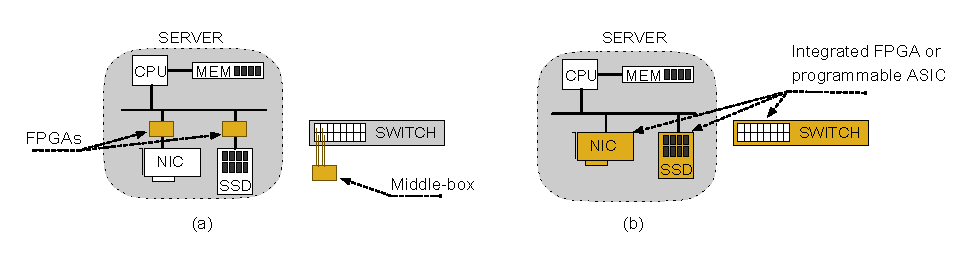
\includegraphics[bb=0 0 451 108]{fig_bump_internal.eps} %% 0.75
    \caption{Alternative in-network computing and near-storage processing
      platforms.
      (a) Using ``bump-in-the-wire'' FPGAs or network ``middle-boxes'' to create
      early application logic sites.
      (b) Leveraging programmability within the device for application logic.}
    \label{fig:bump_internal}
\end{figure}


The networking and storage stacks have always carried some computing power.
Network switches can triage billions of packets per second.
Solid-state drives (SSDs) can scramble and encode gigabytes of data per second
(for error correction purposes~\cite{cai17}).
Despite such computing power, applications have no access to how the
devices process the data, other than by issuing IO requests.
The functionality of these devices has been closed to changes.  Opening them
would require supporting a certain level of \emph{programmability}.


Nonetheless, the benefits of executing application logic close to networking and
storage devices are known~\cite{fang19, teubner13}.
New algorithms that take advantage of proximity to the data become viable and
provide both performance and power consumption gains.
Figure~\ref{fig:bump_internal}(a) illustrates how FPGAs and network
``middle-boxes'' can create these opportunities.


The lack of programmability in network and storage devices has impacted not
only applications.
It has also hindered the advancement of these platforms.
On the networking side, new protocols emerge that depend heavily on hardware to
run at high-speeds.
\emph{Fixed-function} devices, the ones that have their functionality ``baked''
into the hardware, may need to undergo a full, lengthy development cycle before
they can run new protocols.
Recently, a solution emerged where a new class of networking devices started
supporting programmability (e.g., in programmable switches~\cite{bosshart13} and
``smart'' NICs~\cite{zilberman14}).
The protocols these devices run are expressed as software programs.


The need for programmability also emerged on storage platforms recently.
SSDs are designed to shield applications from the intricacies of managing
flash memory.
However, evidence appeared that SSDs often miss the right performance decisions
because of the separation between it and the
applications~\cite{bjorling17}.
A more \emph{modular} SSD design, deemed \emph{open-channel}, was proposed that
allows a host (a server), rather than the SSD itself, to make certain low-level
decisions.
The modules that run on the host are software-based, therefore programmable.


Developers soon realized that the programmability could also be used by
applications.
It made it possible to inject application code directly into the networking and
storage stacks.
Figure~\ref{fig:bump_internal}(b) depicts such a scenario.
\emph{In-network computing} and \emph{near-storage processing} emerged as the
disciplines that leverage processing power in the network and storage stacks,
respectively, for application purposes.


An application that benefits from INC or NSP contains, by definition, algorithms
running in different computing elements of a system.
These algorithms ought to communicate at high speed.
The most commonly used interconnect for such systems has been based on the
PCIe bus standard~\cite{budruk03}.
At this time, the standard is being revised to operate at higher speeds.
PCIe is also being extended with mechanisms to support cache coherence protocols
to run atop of it~\cite{ccix19, cxl19}.


Despite their potential, INC and NSP platforms are not without challenges.
INC is a more mature technology with increasingly popular programmable models
that shield the developer from the intricacies of the devices.
Such programming models, however, are quite different from a general-purpose
CPU’s.
In contrast, NSP often uses general-purpose processors---but much less powerful
ones than server-class CPUs.
In both cases, porting algorithms to these platforms requires rethinking the
algorithms to fit either a different model or a less-powerful environment.


In this paper, we elaborate on the above challenges and opportunities of
adopting INC and NSP as platforms to improve application performance.
We summarize the contributions of this paper are as follows:
\begin{itemize}
  \setlength{\itemsep}{0pt}
  \setlength{\parsep}{0pt}
  \setlength{\parskip}{0pt}
  \setlength{\topsep}{0pt}
  \setlength{\partopsep}{0pt}
\item We discuss the evolution and recent advancements of INC and NSP platforms;
\item We present specific computation tasks that can benefit from them;
\item We describe the challenges that still remain in order to use INC and NSP
  as application platforms;
\item Finally, we present the benefits of adopting the current generation of INC
  and NSP.
\end{itemize}


The rest of this paper is structured as follows.
We discuss the programmability of the network and storage stacks in more detail
in Section~\ref{sec:background}.
We show examples of computing paths that can leverage INC and NSP capabilities in
Section~\ref{sec:data_paths}.
We comment on the evolution of the PCIe interconnect and the possibilities it
opens in Section~\ref{sec:interconnects}.
We discuss the challenges and opportunities of adopting INC and NSP platforms in
Section~\ref{sec:challenges}.
We elaborate on how ready for adoption the technologies are in
Section~\ref{sec:discussion}, before concluding in Section~\ref{sec:conclusion}.


\section{An Abridged History of INC and NSP}
\label{sec:background}

There have been many attempts to conciliate speed and flexibility in
networking hardware devices.
Figure~\ref{fig:evolution_net} depicts the main ideas behind the relevant
milestones in that context.


\begin{figure}[h]
  \centering
  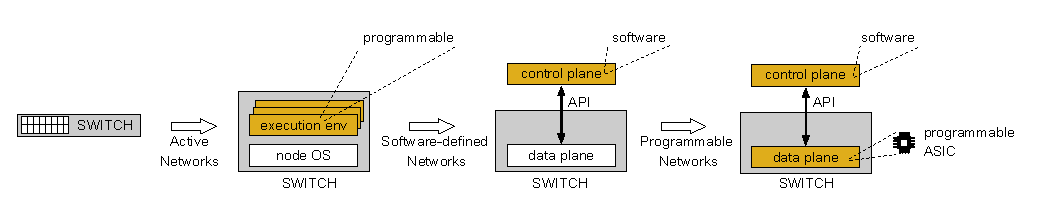
\includegraphics[bb=0 0 483 88]{fig_evolution_net.eps} %% 0.68
  \caption{Evolution of the network stack towards programmability.}
  \label{fig:evolution_net}
\end{figure}


\emph{Active Networks}, one of the first attempts, proposed a standard
architecture for more flexible network devices~\cite{calvert98}.
The goal of the architecture is to enable changes to the device
behavior—--typically to implement new protocols—--via the execution of
user-driven customization.
There are two main components in such a device.
First, a node operating system that manages basic IO functionality, including
processing, storage, and transmission.
Second, multiple Execution Environments (EE) that support the execution of
programs containing packet-processing logic.
Applications can inject code into the device through an API, which generates
special packets for the device to execute.
Active networks proved to be very flexible; however, they ran considerably
slower than their fixed-function counterparts.


\emph{Software-Defined Networks} (SDN), a later attempt at a more flexible
network, is also centered around a standard device
architecture~\cite{kreutz15}.
The main feature of the architecture is the separation of the control plane
(policy definition) from the data plane (policy implementation).
The control plane would contain information such as routing tables; the data
plane would use that information to forward packets without sacrificing speed.
An SDN device could adopt a new protocol if the SDN standard recognizes that
protocol.
Introducing new protocols, however, still required changes in the SDN standard
itself and sometimes also on the devices.
The main issue was that SDN only supports custom logic on the control plane.
Protocols that depended on special per-packet logic need to send these packets
to the control plane, which in turn processes them, pushing the results back to
the data plane.
The additional path cannot sustain \emph{line-rate}, as one calls the individual
port speed of a switch.


In a more recent development, \emph{Programmable Dataplanes} (also referred to
as \emph{Programmable Networks}) allowed custom logic on the data
plane~\cite{bifulco18}.
The cornerstone of this technology is a generation of programmable ASICs (chips)
that supports a certain degree of stateful packet processing without compromising
speed~\cite{bosshart13}.
This balance is captured by a programming model called Protocol Independent
Switch Architecture (PISA)~\cite{sivaraman16}.
PISA shields the programmer from various device intricacies and, because it was
designed to be protocol-independent, it proved adept at expressing application
computations as well.
Programmable networks created the conditions for a new generation of
applications to push specialized logic into the network, i.e., to perform
\emph{in-network computing}.


\vspace{1em}
We now turn our attention to the evolution of the storage stack.
Just as with networks, the idea of near-storage processing is not new, but the
driver for altering this stack has been more application-centric than in
networking.
In the early 2000s, a seminal proposal, called \emph{Active Disks}, gained
traction that aimed at transforming hard drive controllers into data-processing
platforms~\cite{riedel01}.
These controllers often carried a small, general-purpose processor that was
somewhat over-dimensioned for its purpose.
Applications could place logic on that processor, and access/modify the data
blocks that were streaming in and out of the hard drive.
The computing power of these controllers ultimately proved to be underwhelming,
and the industry saw little need to improve them.


Eventually, SSDs based on NAND-flash displaced hard drives in many applications.
Managing flash memory requires considerably more computing power than a magnetic
medium, and flash memory error rates are very high, which requires
computational-intensive error correction techniques~\cite{cai17}.
Moreover, the industry decided that SSDs should be drop-in replacements for hard
drives.
SSDs execute internally a compatibility layer called Flash Translation Layer
(FTL) for that purpose~\cite{chung09}.
All these factors turn SSDs into relatively powerful embedded devices.


A proposal soon emerged to leverage SSD controllers for database query
processing using \emph{smart SSDs}~\cite{do13}.
As with active disks, the computing capacity on early devices was not sufficient
for most computations in practice~\cite{do19}.
It would take a new generation of devices to accommodate fast database
logic~\cite{kim16}.
However, the industry focus was more on making devices faster than on making
them smarter.
Performance wasting was an issue, as the FTL not always makes the best decisions
from an application's point of view.
Some efforts emerged that tried to make SSD architectures more open to
configurations.
Figure~\ref{fig:evolution_ssd} captures the essential steps of this effort.


\begin{figure}[h]
  \centering
  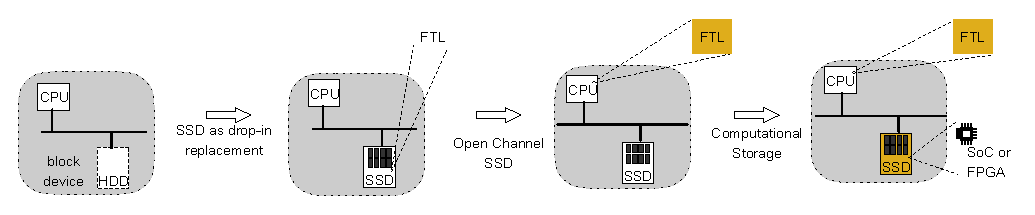
\includegraphics[bb=0 0 481 87]{fig_evolution_ssd.eps} %% 0.68
  \caption{Evolution of the storage stack towards programmability.}
  \label{fig:evolution_ssd}
\end{figure}

\emph{Open Channel SSDs} appeared from a growing understanding that many of the
FTL tasks were better performed leveraging application
knowledge~\cite{bjorling17}.
In an open-channel SSD, some of the FTL responsibilities are removed from the
device.
Instead, they run on the host housing the SSD or even inside individual
applications~\cite{ouyang14}.
Naturally, these devices expose a lower-layer view of the underlying flash
medium.


With more exposure to SSD architectural details, several works emerged to build
tooling around these devices.
These efforts range from frameworks to program SSD controllers~\cite{picoli20},
to performance measurement tooling~\cite{lerner20}, to even full SSD rapid
prototyping platforms~\cite{kwak20}.
At the same time, a class of works appeared that deploy application code on
SSDs, making them a \emph{Computational Storage} platform~\cite{picoli19, ruan19,
woods14}.
The common thread in these works is that they increase the existing computing
power of the devices by building them on platforms such as a System-on-a-Chip
(SoC) or an FPGA.
The tooling and the additional computing capacity paved the way for
\emph{Near-Storage Processing}.


One problem that remains open, however, is the lack of a consensus around a
programming model.
While there are recent proposals in that sense (e.g., in~\cite{gu16}), these
models leave many aspects undefined.
For instance, they have not addressed how to interface application logic with
internal device mechanisms.
An application that wishes to influence the IO scheduling policy of a device
directly has no means to do so.
There is also no consensus on how to shield an application developer from
specific aspects of different devices.


\section{Alternative Computing Paths}
\label{sec:data_paths}

INC and NSP  provide alternative sites beyond a CPU where applications can place
logic.
This fundamentally changes the traditional data movement patterns we see in
CPU-centric algorithms, potentially bringing performance and power savings
benefits.
We illustrate these possibilities in this section by presenting and discussing
several use cases in large-scale data management.


\subsection{In-Network Data Aggregation}
\label{ssec:aggr}

Data aggregation is a very common operation in data management.
Aggregation involves grouping data by specific criteria and calculating
summaries over each group.
A typical example is the \texttt{GROUP BY} clause in \texttt{SQL}.
When the data volume is large, the operation can involve several servers,
e.g., as in a rack-wide computation.
Figure~\ref{fig:flow_1}(a) illustrates one possible way to solve such a distributed
aggregation.


The servers agree on how to partition the data, taking into consideration the
grouping key.
This divides the work into disjoint, independent tasks.
Each server reshuffles its data while performing the aggregation over its
assigned partition, as data arrives.
Eventually, all the machines send their aggregation results to an elected
server, which combines them into a global result.
Note that throughout all these interactions, the switch performs data
transmissions only.


\begin{figure}[h]
    \centering
    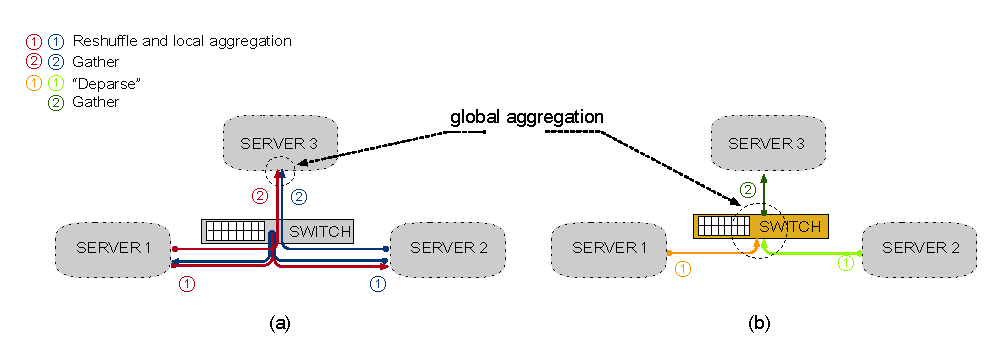
\includegraphics[bb=0 0 462 156]{fig_flow_1.eps} %% 0.75
    \caption{Data aggregation scenario (e.g., SQL GROUP BY).
      (a) With a ``passive'' switch, the servers first repartition the data
      and work on aggregating its assigned partition locally.
      Then, an elected server gathers all partitions and performs the global
      aggregation.
      (b) On an INC platform, an ``active'' switch can, in typical situations,
      perform the global aggregation in one step and transmit the results to an
      elected server.
      We use a given color to represent each unique data stream in the
      computation.
      }
    \label{fig:flow_1}
\end{figure}


In Figure~\ref{fig:flow_1}(b), we show that using the switch as an active
element simplifies the entire computing path~\cite{lerner19}.
We assume that the switch is programmable and that it can be leveraged to hold
an entire aggregation table.
The size of such a table is often manageable, as it is proportional to the
number of groups involved, rather than the size of the dataset.
Note that the servers need not reshuffle the data nor perform an aggregation on
a partition.
Because programmable switches perform computations at line-speed, the
aggregation table on the switch will be completed as soon as the last server
finishes transmitting its tuples, and can then be sent immediately to an elected
server.


Not all computations are suitable for INC deployment.
The important caveats include: (a) the number of steps the switch can execute
over each packet is limited; (b) the kind of instructions the switch can perform
is also constrained; and (c) programmable network devices adhere to a
programming model that imposes a \emph{forward logic}-style onto algorithm
design.
Loops and complex branching are strongly discouraged, although possible.
In practice, these restrictions reduce the choices of data structures the switch
can support.
In particular, the aggregation described in Figure~\ref{fig:flow_1}(b) requires
a hash table to be adapted to INC constraints.
In this case, the number of collisions can be handled on the switch up to a
certain bound.
Relaxing this constraint involves using a technique called
``overflowing''~\cite{lerner19}, which allows treating long collision chains
outside the switch without a noticeable performance penalty in most cases.

These limitations notwithstanding, a large class of computations can benefit from
INC platforms~\cite{ports19}.
Moreover, processing data on the switch tends to scale well as the number of
servers grows in the cluster.
The number of switches naturally grows with the number of servers.


\subsection{Near-Storage Checkpoint Derivation}
\label{ssec:cp_derivation}

We now describe an opportunity that arises specifically in an in-memory database
system.
Like most DBMSs, in-memory databases guarantee durability using a persistent
transaction log.
Because the log can get arbitrarily long, it would be impractical to recover
from a crash just by replaying it.
Therefore, databases also perform a periodical checkpoint (e.g., by taking a
snapshot) of the current memory state and write it to persistent storage, often
SSDs.
A recovery algorithm can load the snapshot and replay the portion of the log
acquired after the checkpoint.
In in-memory databases, the log and checkpoint are the only workloads written to
disk.


The logging and checkpointing processes compete for both disk and memory
bandwidth.
Figure~\ref{fig:flow_2}(a) shows these contention points.
The checkpointing process reads the database contents from the main-memory while
it is being queried/modified.
The checkpointing process also issues write requests to the SSD, which have to
be scheduled along with the logging workload.
The contention is responsible for the throughput reduction that many systems
experience during checkpoints.


\begin{figure}[h]
  \centering
  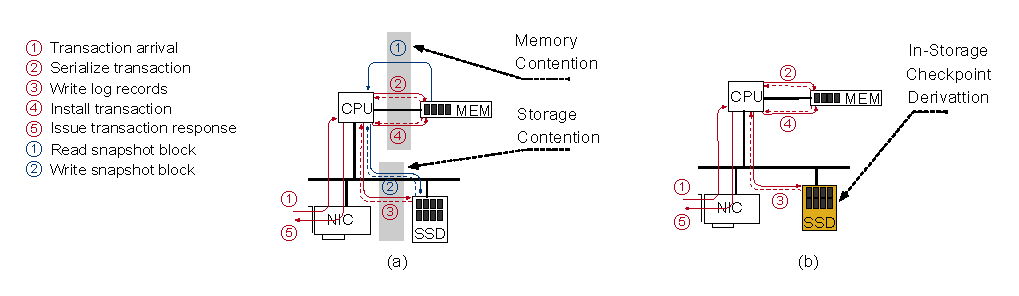
\includegraphics[bb=0 0 473 126]{fig_flow_2.eps} %% 0.75
  \caption{Checkpoint computation scenario.
    (a) Transaction logging (red) and checkpoint (blue) are two parallel
    processes.
    They compete for memory and disk bandwidth.
    (b) A checkpoint could be derived by processing the transaction log inside
    an SSD.
    The solid lines represent data; the dashed ones, control and/or return.
  }
  \label{fig:flow_2}
\end{figure}


The key observation here is that partial snapshots, which can serve as
checkpoints, can be derived from the log stream directly.
We believe that such derivations may very well occur inside a smart SSD.
We show in Figure~\ref{fig:flow_2}(b) that once we move that process to the
device, the contention points disappear.


Note, however, that the processing power on an SSD is far smaller than that of a
general-purpose CPU.
We cannot possibly expect to move the same algorithm we used on a CPU into an
NSP platform and obtain similar performance results.
Creating a checkpoint derivation algorithm for an SSD requires finding snapshot
approximations that the device can process at the necessary pace.
We comment on Section~\ref{sec:challenges} how specific architectural changes on
smart SSDs can make this task easier.


\subsection{Low Latency Database Replication}
\label{ssec:low_latency}


Another code path that can benefit from either INC or NSP is that of a replica
node in a database system.
On a master node, transactions need to be serialized via a concurrency control
algorithm.
The latter typically runs on a CPU.
The replica node code-path is simpler because the serial order of the
transactions was already determined.
The CPU takes the modifications coming from the network card and persists them
on disk in the same order it received them.
Subsequently, it updates its data structures and sends a notification to the
master node that it accepted the transaction.
Figure~\ref{fig:flow_3}(a) depicts such an interaction.


\begin{figure}[h]
  \centering
  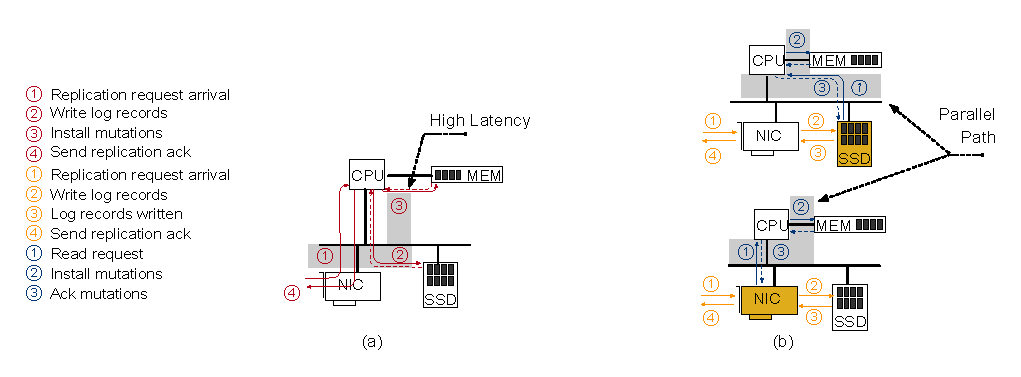
\includegraphics[bb=0 0 474 165]{fig_flow_3.eps} %% 0.75
  \caption{Database replica node scenario.
    (a) Each transaction log entry is first persisted in storage and then
    applied to memory, as the CPU coordinates the replication.
    (b) If an ``active'' NIC or SSD coordinates the process, the persistence and
    memory update paths can proceed in parallel.
  }
  \label{fig:flow_3}
\end{figure}


Note that the replica code path incurs in latency.
The master node may be withholding the original transaction until the
replication path is completed.
We can optimize this code path in at least two ways.
Using NSP, the NIC would send the modification stream directly to a smart SSD.
In turn, the SSD could be programmed to coordinate the interaction instead of
the CPU.
The SSD would notify the NIC after it persisted the changes, reducing the
latency.
It would also, in parallel, allow the CPU to read (and perform) the
modifications.
An alternative path exists where the NIC itself would perform the coordination.
Figure~\ref{fig:flow_3}(b) shows both cases.
This scenario involves having the NIC and the SSD communicate without any CPU
intervention.
This type of communication is called peer-to-peer DMA~\cite{budruk03} and it has
been used in other contexts before, such as direct access to a remote disk
(e.g., NVMe-over-Fabrics~\cite{guz18}).


\section{Upcoming Interconnects}
\label{sec:interconnects}

INC and NSP platforms rely on an interconnect to communicate with other
computing elements in a system.
PCIe has been the \emph{de facto} interconnect for quite a
while~\cite{budruk03}.
PCIe is a point-to-point bus with a variable number of lanes dedicated to
devices.
Each lane can transfer close to 1GB/s on the current standard version, Gen 3.
Cards attached to the bus can use 1$\times$, 2$\times$, 4$\times$, 8$\times$, or
16$\times$ lanes to achieve a theoretical maximum of 16 GB/s bidirectional
bandwidth.


Newer devices are creating the need for faster speeds.
For instance, the standard NIC port speeds are about to go from 100 Gb/s to 400
Gb/s, which a single Gen 3 PCIe slot can no longer support.
The PCIe standard had moved to 2 GB/s lanes on Gen 4.
The following iteration of the standard, Gen 5, brings 4 GB/s lanes with a
theoretical bi-directional bandwidth of 64GB/s for 16$\times$ device.


There is another compelling feature that new versions of PCIe buses will bring:
cache coherence.
This feature allows computing elements to negotiate who may be caching a given
portion of memory at any given time.
It also determines who has the license to write to that memory address.
Coordinating access to single memory address allows all the computing elements
to share a single view of memory, as Figure~\ref{fig:coherence}(a) shows.
There are two flavors of coherency: one in which the CPU has a prominent role in
controlling the memory, called \emph{asymmetric}, and one in which all computing
elements play a similar role, called \emph{symmetric}.


\begin{figure}[h]
  \centering
  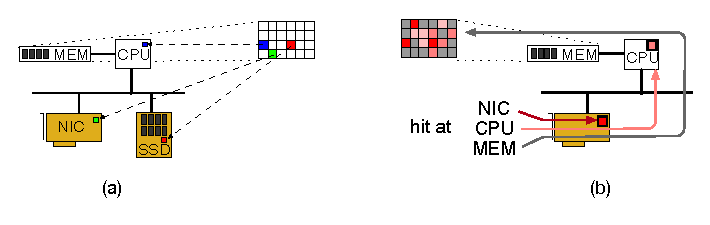
\includegraphics[bb=0 0 325 92]{fig_coherence.eps} %% 0.75
  \caption{Cache coherency scenarios: (a) a NIC and an SSD may be responsible
    for writing to specific addresses in memory that can be read by other
    elements, and (b) a NIC can be responsible for caching (and writing to) very
    hot pages while leaving the CPU responsible for less accessed pages.
  }
  \label{fig:coherence}
\end{figure}


At the time of writing, there are four upcoming interconnects offering both high speed and coherence:
CAPI~\cite{stuecheli15}, CCIX~\cite{ccix19}, CXL~\cite{cxl19} and
Gen-Z~\cite{knebel19}.
CCIX and Gen-Z support symmetric coherence, unlike CAPI or CXL, which support
asymmetric coherence.
CAPI is a competing standard to PCIe.
CCIX and CXL use only PCIe, while Gen-Z can use ethernet as well as PCIe.
The range of PCIe is short enough to work only within the confines of a chassis,
while ethernet allow to connect across chassis.
This opens up the possibility of CCIX or CXL being applied simultaneously with
Gen-Z to form coherence domains that cross server boundaries.


Cache coherency allows for new INC and NSP design use cases.
For instance, one may extend the caching hierarchy beyond the CPU.
Figure~\ref{fig:coherence}(b) illustrates this possibility.
Some distributed applications may cache hot data items in the
NIC~\cite{tokusashi18}.
With coherence, the NIC can also request write access to such an item and update
it.
Any other computing element that requests to cache that address would then see
the updates.


\section{Challenges and Opportunities}
\label{sec:challenges}

We mentioned above some immediate difficulties that arise when deploying current
generation INC and NSP platforms.
In this section, we elaborate on further challenges and opportunities that we
believe would unlock more of the potential of these platforms.


\softsubsec{In-Network Stateful Computations.}
%
Data management primarily involves stateful computations, i.e., algorithms that
access a result from a previous iteration and generate a new result at the
next one.
The aggregation operation discussed in Section~\ref{ssec:aggr} is one such
algorithm.
Maintaining state in-network, particularly in switches, is currently very
challenging.
Programmable switches rely on high-speed memories that, for cost reasons, are
present in limited amounts.
Moreover, switches have a very strict ``allowance'' of how many instructions
they can execute per packet and what those instructions can do.
These restrictions make maintaining data structures other than a hash
table on a switch possible but difficult.
Even some common operations on hash tables, such as collision management,
require some adapting, as we discussed above.


We miss a computing model that can relax those restrictions to a certain extent
while still keeping the ability to run logic at line-speed.
Supporting such a model would most likely require introducing new hardware onto
programmable switches.
We believe such a model is possible, but the field of in-network computing is
still new.
There is not yet a clear list of missing operations from applications beyond
networking protocols on which to base new switch hardware capabilities.


\softsubsec{SSD-Application Interface.}
%
A regular SSD makes several decisions such as IO scheduling and page mapping
based solely on observing the stream of IO commands it receives~\cite{nam11}.
When application logic executes inside the device, it becomes an additional
stream of IO commands.
The internal and external streams would likely compete with one another.
A straightforward way to manage the new internal streams is to pretend they came
from outside and to proceed as usual.


An alternative way would be to allow the application logic and the device to
interact.
Consider again the checkpoint derivation scenario we describe in
Section~\ref{ssec:cp_derivation}.
It generates new IO requests at a given pace.
Depending on the current load on the SSD, the checkpoint stream can be too fast or
too slow for the device to handle.
Ideally, we want a means for the device and the application logic to negotiate
that pace.
There is an opportunity here to establish a communication model that supports
this kind of interaction.


\softsubsec{SSD Channel Architecture.}
%
An SSD's bandwidth and capacity are a result of combining many relatively
limited NAND flash \emph{packages} (chips)~\cite{micheloni12}.
A typical arrangement is to group the packages in disjoint sets called
\emph{channels}.
There are anywhere between 8 to 32 channels in a typical SSD.
This arrangement has proved adequate when data pages are transferred in and out
of the device.


The introduction of application logic into an SSD, however, can cause data
pages to be moved \emph{across packages}---possibly between channels.
For instance, we describe in Section~\ref{ssec:cp_derivation} how an NSP process
can read pages from a transaction log and write them, after some manipulation,
as pages of a checkpoint.
In a traditional SSD architecture, this pattern would consume bandwidth from
both the origin and the destination channels.
We believe that there may be other package interconnect architectures
beyond channels that are more suited to the data movements above.
To the best of our knowledge, there has been no study about interconnects that
involve architectures other than fixed channels.


\softsubsec{Code-Variant Generation and Selection.}
%
INC and NSP platforms introduce additional hardware heterogeneity to computing
platforms.
An algorithm implementation that works well on a given switch may not work on a
different one, due to architectural differences.
The generation and selection of variant implementations is a known problem; it
appeared before in domains such as GPUs~\cite{rosenfeld15}.


To complicate matters, some algorithms are flexible enough to be deployed either
on a NIC or on the switch to which it connects.
The selection of the most appropriate platform constitutes an optimization step
that compounds to the variant selection problem above.
Currently, the programmer is responsible for making such choices.
There is an opportunity for creating higher-level tooling that would aid in
these decisions.


\softsubsec{Runtime Resource Management.}
%
In a regular setting, the operating system mediates every single network and
storage IO between applications and devices.
The OS does so by interposing itself between the two.
What, then, should be the role of the OS when a portion of the applications
reside \emph{inside} the device?


One potential solution is to accept that applications may want to access a device
directly, without mediation.
Such is the premise of Arrakis~\cite{peter15}, which tricks an application into
interacting with virtual versions of the devices, and redesigns the kernel to
provide the expected protections under such assumptions.


\section{Discussion}
\label{sec:discussion}

Notwithstanding the challenges and opportunities described in the previous
section, INC and NSP platforms are a reality.
The question arises as to whether they are ready for adoption.
In this section, we break this question into a list of sub-questions and answer
each one in turn.


\softsubsec{Are there diverse offerings of INC and NSP platforms?}
%
INC can be realized by many different hardware targets, both on switches and
NICs.
In terms of programmable switches, there are at least three silicon
manufacturers producing programmable ASICs: Barefoot (Intel)
Tofino~\cite{barefoot}, Broadcom Trident 4~\cite{broadcomT4}, and Cavium
(Marvel) Xpliant~\cite{cavium}.
Together, these chips appear in several commercial offerings from companies such as
Cisco and Arista.
SmartNICs are also widely available, ranging from FPGA-centric accelerators such as
Xilinx Alveo~\cite{xilinx} to more software-oriented platforms such as
Netronome~\cite{netronome}.
The offering for programming languages and abstractions is also diverse.
A prevalent language is \texttt{P4}~\cite{bosshart14}, but there are variations
such as \texttt{NPL}~\cite{broadcomnpl} and even \texttt{C} libraries in some
cases~\cite{netronome}.


NSP is also a rich environment with many prototyping and commercial platforms
available.
For instance, SSDs are starting to emerge that introduce application
specializations.
Samsung has recently announced the KV-SSD, which incorporates Key Value store
logic within its firmware~\cite{ki17}.
One issue with such offerings is that they add application functionality
but do not expose programmability.
The interested reader should look at~\cite{picoli20} for an extensive list of
specialized SSD and NSP-platforms available at the time of writing.


\softsubsec{What are the advantages of INC and NSP compared to ``CPU-centric''
alternatives?}
%
While there is no study yet of an exacale platform that resorts to both INC and
NSP, the expected benefits are a combination of increased performance, lower
energy expenditure, and lower CPU utilization.
There a numerous works that provide partial results.

For INC, data manipulations such as the one described in Section~\ref{ssec:aggr}
were studied before~\cite{lerner19}.
We can expect to see the performance of many typical queries improve by a factor of
2$\times$\ by using programmable switches at moderate network
speeds.
The power consumption in these switches is estimated to be only 12.4\% higher
than their fixed-function counterparts, and, anecdotally, the switches cost
about the same.
The operations-per-Watt ratio on some INC platforms such as smartNICs was
also studied before~\cite{tokusashi18}.
For instance, a variant of the caching scenario we discussed in
Section~\ref{sec:interconnects} reports a 17$\times$ better power utilization as
compared to a regular CPU.


NSP platforms deliver similar benefits.
According to~\cite{kim16}, the performance of scans and joins can see
performance improvements between 5$\times$ and 47$\times$, the cost of equipping
an SSD to support near-storage processing is less than 1\% of its total cost,
and the energy-efficiency compared to performing those operations on a CPU can be up
to 45$\times$ better.


\softsubsec{Are there standards in place to guarantee the portability and
longevity of the solutions?}
%
There is a big difference from a standardization point of view between INC and
NSP technologies.
As mentioned above, INC has broadly embraced \texttt{P4} as a programming language.
The latest edition of the language, \texttt{P4$_{16}$}, allows different target
platforms to express their capabilities.
A compiler can generate specific code from a unique source to different, maybe
even disparate, devices.
These feature makes the language flexible enough to work on future devices,
which can only help its adoption.


In contrast, there is not yet a consensus on how computational storage should be
programmed.
We even miss a standard around what an open-channel SSD should be, which would
arguably be a necessary step.


\section{Conclusion}
\label{sec:conclusion}

In this paper, we reviewed how the evolution of the network and storage stacks
have unlocked their computing power.
Applications can not only request services from these stacks, but also
embed logic into them.
We showed that with a careful redesign, algorithms running on INC or NSP
platforms could present a reduced amount of data movement, lower CPU
utilization, less energy consumption, or a combination of these.


We also discussed several challenges that INC and NSP still face.
Despite these limitations, we commented on a current generation of INC- and
NSP-enabled devices that are available off-the-shelf.
We believe that the emergence of the network and storage stacks as computing
elements creates promising ways to scale typical data management computations.


\softsec{Acknowledgments.}
%
This project has received funding from the European Research Council (ERC) under
the European Unions Horizon 2020 research and innovation programme (grant
agreement 683253/GraphInt).


\begin{thebibliography}{10}
\itemsep=1pt
\begin{small}

\bibitem{barefoot}
  \newblock Barefoot Tofino and Tofino 2 Switches.
  \newblock https://www.barefootnetworks.com/products/brief-tofino-2/.

\bibitem{bifulco18} R.~Bifulco, and G.~R\'etv\'ari.
  \newblock A Survey on the Programmable Data Plane: Abstractions, Architectures, and Open Problems.
  \newblock {\em HPSR}, June, 2018.

\bibitem{bjorling17} M.~Bj{\o}ling, J.~Gonz\'alez, and P.~Bonnet.
  \newblock Lightnvm: The Linux Open-Channel SSD Subsystem
  \newblock {\em FAST}, February, 2017.

\bibitem{broadcomnpl} Broadcom NPL.
  \newblock Network Programming Language.
  \newblock {\em https://nplang.org/}.

\bibitem{broadcomT4} Broadcom.
  \newblock Broadcom Trident 4.
  \newblock {\em https://www.broadcom.com/products/ethernet-connectivity/switching/strataxgs/bcm56880-series}.

\bibitem{bosshart13} P.~Bosshart, G.~Gibb, H.-S.~Kim, G.~Varghese, N.~McKeown, M.~Izzard, F.~Mujica, and M.~Horowitz.
  \newblock Forwarding Metamorphosis: Fast Programmable Match-Action Processing in Hardware for SDN.
  \newblock {\em SIGCOMM CCR}, 43(4):99--110, 2013.

\bibitem{bosshart14} P.~Bosshart., D.~Daly, G.~Gibb, M.~Izzard, N.~McKeown, J.~Rexford, C.~Schlesinger, D.~Talayco, A.~Vahdat, G.~Varghese, and D.~Walker.
  \newblock P4: Programming protocol-independent packet processors.
  \newblock {\em ACM SIGCOMM CCR}, 44(3):87--95, 2014.

\bibitem{budruk03} R.~Budruk, D.~Anderson, and E.~Solari.
  \newblock PCI Express System Architecture.
  \newblock {\em Pearson Education}, 2003.

\bibitem{cai17} Y.~Cai, S.~Ghhose, E.F.~Haratsch, Y.~Luo, and O.~Mutlu.
  \newblock Error Characterization, Mitigation, and Recovery in Flash-Memory-Based Solid-State Drives.
  \newblock {\em Proc. of the IEEE}, 105(9), 1666--1704, 2017.

\bibitem{calvert98} K.L.~Calvert, S.~Bhattacharjee, E.~Zegura, and J.~Sterbenz.
  \newblock Directions in Active Networks.
  \newblock {\em IEEE Comm. Magazine}, 36(10):72--78, 1998.

\bibitem{cavium} Cavium.
  \newblock XPliant Ethernet Switch Product Family.
  \newblock {\em www.cavium.com/XPliant-Ethernet-Switch-Product-Family.html}

\bibitem{ccix19} CCIX Consortium.
  \newblock An Introduction to CCIX.
  \newblock {\em White Paper}, https://www.ccixconsortium.com/wp-content/uploads/2019/11/CCIX-White-Paper-Rev111219.pdf

\bibitem{chung09} T.-S.~Chung, D.-J.~Park, S.~Park, D.-H.~Lee, S.-W.~Lee, and H.-J.~Song.
  \newblock A Survey of Flash Translation Layer.
  \newblock {\em J. of Syst. Archit.}, 55(5--6):332--343, 2009.

\bibitem{cxl19} D.D.~Sharma.
  \newblock An Introduction to Compute Express Link.
  \newblock {\em White Paper}, https://docs.wixstatic.com/ugd/0c1418\_d9878707bbb7427786b70c3c91d5fbd1.pdf.

\bibitem{do13} J.~Do, Y.S.~Kee, J.M.~Pzatel, C.~Park, K.~Park, and D.J.~DeWitt.
  \newblock Query Processing on Smart SSDs: Opportunities and Challenges.
  \newblock {\em SIGMOD}, June, 2013.

\bibitem{do19} J.~Do, S.~Sengupta, and S.~Swanson.
  \newblock Programmable Solid-State Storage in Future Could Datacenters.
  \newblock {\em CACM}, 62(6):54--62, 2019.

\bibitem{fang19} J.~Fang, Y.T.B.~Mulder, J.~Hidders, J.~Lee, and H.P.~Hofstee.
  \newblock In-Memory Database Acceleration on FPGAs: A Survey.
  \newblock {\em VLDB Journal}, October, 2019.

\bibitem{gu16} B.~Gu, A.S.~Yoon, D.H.~Bae, I.~Jo, J.~Lee, and J.~Yoon.
  \newblock Biscuit: A Framework for Near-Data Processing of Big Data Workloads.
  \newblock {\em SIGARCH Comp. Arch. News}, 44(3):153--165.

\bibitem{guz18} Z.~Guz, H.~Li, A.~Shayesteh, and V.~Balakrishnan.
  \newblock Performance Characterization of NVMe-over-Fabrics Storage Disaggregation.
  \newblock {\em ACM Trans. on Storage}, 14(4):1553--3077, 2018.

\bibitem{ki17} Y.-S.~Ki.
  \newblock Key Value SSD Explained – Concept, Device, System, and Standard.
  \newblock {\em SNIA SDC}, September, 2017.

\bibitem{kim16} S.~Kim, H.~Oh, C.~Park, S.~Cho, S.-W.~Lee, and B.~Moon.
  \newblock In-Storage Processing of Database Scans and Joins.
  \newblock {\em Inf. Sci.}, 327(C):183--200, 2016.

\bibitem{knebel19} P.~Knebel, D.~Berkram, A.~Davis, D.~Emmot, P.~Faraboschi, and G.~Gostin.
  \newblock Gen-Z Chipset for Exascale Fabrics.
  \newblock {\em HotChips}, August, 2019.

\bibitem{kreutz15} D.~Kreutz, F.M.V.~Ramos, P.E.~Ver\'issimo, C.E.~Rothenberg, S.~Azodolmolky, and S.~Uhlig.
  \newblock Software-Defined Networking: A Comprehensive Survey.
  \newblock {\em Proc. of the IEEE}, 103(1):14--76, 2015.

\bibitem{kwak20} J.~Kwak, S.~Lee, K.~Park, J.~Jeong, and Y.H.~Song.
  \newblock Cosmos+ OpenSSD: Rapid Prototype for Flash Storage Systems.
  \newblock {\em ACM Trans. on Storage}, to appear.

\bibitem{lerner19} A.~Lerner, R.~Russein, and P.~Cudr\'e-Mauroux.
  \newblock The Case for Network Accelerated Query Processing.
  \newblock {\em CIDR}, January, 2019.

\bibitem{lerner20} A.~Lerner, J.~Kwak, S.~Lee, K.~Park, Y.H.~Song, and P.~Cudr\'e-Mauroux.
  \newblock It Takes Two: Instrumenting the Interaction between In-Memory Databases and Solid-State Drives.
  \newblock {\em CIDR}, January, 2020.

\bibitem{micheloni12} R.~Micheloni, A.~Marelli, and S.~Eshghi.
  \newblock Inside Solid State Drives (SSDs).
  \newblock {\em Springer}, 2012.

\bibitem{nam11} E.H.~Nam, B. S. J.~Kim, H.~Eom, and S. L.~Min.
  \newblock Ozone (O3): An Out-of-Order Flash Memory Controller Architecture.
  \newblock {\em IEEE Transactions on Computers}, 60(5):653--666, 2011.

\bibitem{netronome} Netronome.
  \newblock Agilio CX SmartNICs.
  \newblock {\em https://www.netronome.com/products/agilio-cx/}

\bibitem{ouyang14} J.~Ouyang, S.~Lin, S.~Jiang, Z.~Hou, Y.~Wang, and Y.~Wang.
  \newblock SDF: Software-Defined Flash for Web-Scale Internet Storage Systems.
  \newblock {\em ASPLOS}, 2014.

\bibitem{peter15} S.~Peter, J.~Li, I.~Zhang, D.R.K.~Ports, D.~Woos, A.~Krishnamurthy, T.~Anderson, and T.~Roscoe.
  \newblock Arrakis: The Operating System Is the Control Plane.
  \newblock {\em ACM TOCS}, 33(4), 2015.

\bibitem{picoli19} I.L.~Picoli, P.~Bonnet, and P.~T\"oz\"un.
  \newblock LSM Management on Computational Storage.
  \newblock {\em DaMoN}, July, 2019.

\bibitem{picoli20} I.L.~Picoli, N.~Hedam, P.~Bonnet, and P.~T\"oz\"un.
  \newblock Open-Channel SSD (What Is It Good For).
  \newblock {\em CIDR}, January, 2020

\bibitem{ports19} D.R.K.~Ports, and J.~Nelson.
  \newblock When Should The Network Be The Computer.
  \newblock {\em HotOS}, May, 2019.

\bibitem{riedel01} E.~Riedel, C.~Faloutsos, G.A.~Gibson, and D.~Nagle.
  \newblock Active Disks for Large-Scale Data Processing.
  \newblock {\em IEEE Computer}, 34(6):68--74, 2001.

\bibitem{rosenfeld15} V.~Rosenfeld, M.~Heimel, C.~Viebig, and V.~Markl.
  \newblock The Operator Variant Selection Problem on Hetergoneous Hardware.
  \newblock {\em ADMS}, August, 2015.

\bibitem{ruan19} Z.~Ruan, T.~He, and J.~Cong.
  \newblock INSIDER: Designing In-Storage Computing System for Emerging High-Performance Drive.
  \newblock {\em Usenix ATC}, July, 2019.

\bibitem{sivaraman16} A.~Sivaraman, A.~Cheung, M.~Budiu, C.~Kim, M.~Alizadeh, H.~Balakrishnan, G.~Varghese, N.~McKeown, and S.~Licking.
  \newblock Packet transactions: High-level programming for line-rate switches.
  \newblock {\em SIGCOMM}, August, 2016.

\bibitem{stuecheli15} J.~Stuecheli, B.~Blaner, C.R.~Johns, and M.S.~Siegel.
  \newblock CAPI: A Coherent Accelerator Processor Interface.
  \newblock {\em IBM Journal of Research and Development}, 59(1):1--7, 2015.

\bibitem{teubner13} J.~Teubner, and L.~Woods.
  \newblock Data Processing on FPGAs.
  \newblock {\em Morgan \& Claypool Publishers}, 2013.

\bibitem{tokusashi18} Y.~Tokusashi, H.~Matsutani, and N.~Zilberman.
  \newblock LaKe: The Power of In-Network Computing.
  \newblock {\em ReConFig}, December, 2018.

\bibitem{xilinx} Xilinx.
  \newblock ALVEO Adaptable Accelerator Cards for Data Center Workloads.
  \newblock {\em https://www.xilinx.com/content/xilinx/en/products/boards-and-kits/alveo.html}

\bibitem{woods14} L.~Woods, Z.~Istv\'an, and G.~Alonso.
  \newblock Ibex: An Inteligent Storage Engine with Support for Advanced SQL Offloading.
  \newblock {\em Proc. of the VLDB}, 7(11):963--974.

\bibitem{zilberman14} N.~Zilberman, Y.~Audzevich, G.A.~Covington, and A.W.~Moore.
  \newblock NetFPGA SUME: Towards 100 Gbps as Research Commodity.
  \newblock {\em IEEE Micro}, 34(5):32--41, 2014.

\end{small}
\end{thebibliography}

\end{document}
